\documentclass[DIV16,BCOR1cm,10pt,a4paper,fleqn,twoside]{scrreprt}         % for pdf output
%\documentclass[DIV16,BCOR1cm,10pt,a4paper,fleqn]{scrreprt}         % for pdf output
%\documentclass[DIV16,BCOR1cm,11pt,a4paper,fleqn]{report}         % for pdf output

% To allow automatic selection of the right graphics type ...
% preset \pdfoutput for older latex installation, it is allways definted for
% news ones
\ifx\pdfoutput\undefined
\gdef\pdfoutput{0}
\fi

\newif\ifpdfx
\ifnum\pdfoutput=0
% latex is called for dvi output
   \pdfxfalse
   \usepackage{graphicx}
\else
% pdflatex is called for pdf output
   \pdfxtrue
   \usepackage[pdftex]{graphicx}
   \usepackage[pdftex]{hyperref}
\fi

\usepackage{textcomp}

%\newcommand{\CDO}{{\bfseries\sffamily CDO\ }}
\newcommand{\CDO}{{\bfseries\sffamily CDO}}
\newcommand{\cdologo}{
\includegraphics{logo/cdo_logo}}

\graphicspath{{figures/}}

% To define headers and footers
\usepackage{fancyhdr}
\pagestyle{fancy}

% Headers and footers personalization using the `fancyhdr' package
\fancyhf{} % Clear all fields

\renewcommand{\headrulewidth}{0.2mm}
\renewcommand{\footrulewidth}{0.2mm}

\renewcommand{\chaptermark}[1]{\markboth{#1}{}}
\renewcommand{\sectionmark}[1]{\markright{#1}}

%\renewcommand{\chaptermark}[1]{\markboth{#1}{}}
%\renewcommand{\sectionmark}[1]{\markleft{#1}}

\fancyhead[LO,RE]{\slshape \leftmark}
\fancyhead[LE,RO]{\slshape \rightmark}
\fancyfoot[LE,RO]{\Large\thepage}
%\fancyfoot[LO,RE]{\raisebox{-2.8mm}{\scalebox{0.17}{\cdologo}}}
\fancypagestyle{plain}{%
  \fancyhead{} % get rid of headers
  \renewcommand{\headrulewidth}{0pt}
}

%\setlength{\footnotesep}{0cm}
%\setlength{\footskip}{-2cm}
%\renewcommand{\footnoterule}{\rule{0cm}{0cm}}

\usepackage{exscale}
\usepackage{array,colortbl}    % color table

\usepackage{listings}
\usepackage{longtable}
\usepackage{color}
\definecolor{pcolor1}{rgb}{0.992, 0.980, 0.875}  % rgb: 253/250/223
\definecolor{pcolor2}{rgb}{1.000, 0.925, 0.700}  % rgb: 255/236/278
\definecolor{pcolor3}{rgb}{0.968, 0.756, 0.623}  % rgb: 247/193/159

%\usepackage{ae}               % fuer die "almost european" computer modern fonts
%\usepackage{url}              % Standard-Paket fuer WWW-Adressen

%\typearea{10}                 % Einen sinnvollen Satzspiegel aktivieren


%Usage:
%pdflatex cdo.tex
%pdflatex cdo.tex
%cat > cdo.ist << 'EOF'
%delim_0        "{\\idxdotfill} "
%headings_flag  1
%heading_prefix "{\\centerline {\\Large \\bf "
%heading_suffix "}}"
%EOF
%makeindex -s cdo.ist cdo.idx
%pdflatex cdo
%thumbpdf cdo
%pdflatex cdo


\usepackage{thumbpdf}

%\usepackage{html}

\usepackage{makeidx}

%\ifpdf
%\usepackage[a4paper, colorlinks=true, pdfstartview=FitV, bookmarks=true, linkcolor=blue,
%            citecolor=blue, urlcolor=blue, latex2html=true]{hyperref}
%\fi

\usepackage{hyperref}
\hypersetup{pdftoolbar=true,
            pdfmenubar=true,
            pdfwindowui=true,   
%            pdffitwindow=true,
            pdfauthor={Uwe Schulzweida},
            pdftitle={CDO Climate Data Operators},
            pdfcreator={pdflatex + hyperref},
            pdfstartview=FitV,
%            pdfpagemode=FullScreen,
            a4paper,
            bookmarks=true,
            linkcolor=blue,
            citecolor=blue,
            urlcolor=blue,
            colorlinks=true}

\setlength{\parindent}{0em}
\setlength{\parskip}{1.5ex plus0.5ex minus0.5ex}
\extrarowheight1pt

\makeindex
%\newcommand{\ii}[1]{\textit{#1}}  \newcommand{\nn}[1]{#1n}
%\renewcommand{\dotfill}{\leaders\hbox to 5p1{\hss.\hss}\hfill}
%\newcommand{\idxdotfill}{5p1{\hss.\hss}\hfill}
\newcommand{\idxdotfill}{\ \dotfill \ }
%\def\idxdotfill{\leaders\hbox to.6em{\hss .\hss}\hskip 0pt plus 1fill}
%\MakeShortVerb{\@}

\renewcommand{\indexname}{Operator index}

\newenvironment{defalist}[1]
{\begin{list}{}
{\settowidth{\labelwidth}{#1\ \ }
\setlength{\itemsep}{0mm}
\setlength{\itemindent}{0mm}
%\setlength{\listparindent}{25mm}
\setlength{\leftmargin}{\labelwidth}
%\setlength{\leftmargin}{25mm}
\setlength{\labelsep}{2mm}
\addtolength{\leftmargin}{\labelsep}
%\addtolength{\leftmargin}{8mm}
}}
{\end{list}}

\newenvironment{defalist2}[1]
{\begin{list}{}
{\settowidth{\labelwidth}{#1\ \ }
\setlength{\itemsep}{0mm}
\setlength{\itemindent}{0mm}
%\setlength{\listparindent}{25mm}
\setlength{\leftmargin}{\labelwidth}
%\setlength{\leftmargin}{25mm}
\setlength{\labelsep}{2mm}
\addtolength{\leftmargin}{\labelsep}
\addtolength{\leftmargin}{8mm}
}}
{\end{list}}

\newcommand{\miniwidth}{\textwidth}

\setcounter{secnumdepth}{3}

\begin{document}


\begin{titlepage}
\vspace*{50mm}
{\Huge{\bf Climate indices with \CDO}}

\setlength{\unitlength}{1cm}
\begin{picture}(16,0.4)
\linethickness{1.5mm}
%\put(0,0.1){\line(1,0){15.85}}
\put(0,0.1){\line(1,0){16.3}}
\end{picture}
\begin{flushright}
\large\bf{Climate indices of daily temperature and precipitation extremes \\ October 2014}
\end{flushright}

\vfill

\Large{\bf Uwe Schulzweida -- \sl MPI for Meteorology}

\Large{\bf Ralf Quast -- \sl Brockmann Consult}

\begin{picture}(16,1)
\linethickness{1.0mm}
%\put(0,0.7){\line(1,0){15.85}}
\put(0,0.7){\line(1,0){16.3}}
\end{picture}
\end{titlepage}

\tableofcontents

\chapter{Introduction}

The Climate Data Operators ({\CDO}) software is a collection of operators
for standard processing of climate and forecast model data.

This document describes additional {\CDO} operators to compute climate indices
of daily temperature and precipitation extreme.
The definition of these climate indices are from the European Climate
Assessment (ECA) project.

The climate indices were implemented in {\CDO} by Ralf Quast
(Brockmann Consult) on behalf of the Service Gruppe Anpassung (SGA) in 2006.
SGA was part of the Model and Data Group (M\&D) at the MPI for Meteorology.
In 2010, the Model and Data Group became the Data Management
department at DKRZ (Deutsches Klimarechenzentrum) and the SGA was
disintegrated. 
For this reason there is no further user support available for these {\CDO} operators.


%\chapter{\label{refman}ECA indices of extremes}
\chapter{\label{refman}Climate indices reference manual}

This section gives a description of all {\CDO} operators to compute the climate indices of daily temperature and precipitation extreme.
Related operators are grouped to modules.
For easier description all single input files are named {\tt ifile} or {\tt ifile1}, {\tt ifile2}, etc.,
and an arbitrary number of input files are named {\tt ifiles}.
All output files are named {\tt ofile} or {\tt ofile1}, {\tt ofile2}, etc.
Further the following notion is introduced:
\begin{defalist}{{\em o(t,x)}}
\item[\(i(t)\)\hfill]
Timestep \(t\) of {\tt ifile}
\item[\(i(t,x)\)\hfill]
Element number \(x\) of the field at timestep \(t\) of {\tt ifile}
\item[\(o(t)\)\hfill]
Timestep \(t\) of {\tt ofile}
\item[\(o(t,x)\)\hfill]
Element number \(x\) of the field at timestep \(t\) of {\tt ofile}
\end{defalist}

%A field is a horizontal slice of a variable on a spezific level.
%The number of elements is the size of the grid.
%It has at least one datapoint. The rank of a field is 1 or 2, this depends
%on the type of the grid.

%A variable is a collection of all fields on different vertical levels
%of the same spezies. Each variable has at least on level. Variable
%with only one level are called 2D variables and all other are 3D variables.

\hspace{3mm}

%\newpage
%\section{Climate indices of daily temperature and precipitation extremes}
%This section contains modules to compute the climate indices
of daily temperature and precipitation extremes.


\input{ref_list_climat}
\input{ref_man_climat}


\begin{thebibliography}{xx}


\bibitem[CDI]{CDI} \ \\
  \href{https://code.mpimet.mpg.de/projects/cdi}
       {Climate Data Interface},
  from the
  \href{http://www.mpimet.mpg.de}
       {Max Planck Institute for Meteorologie}


\bibitem[CDO]{CDO} \ \\
  \href{https://code.mpimet.mpg.de/projects/cdo}
       {Climate Data Operators},
  from the
  \href{http://www.mpimet.mpg.de}
       {Max Planck Institute for Meteorologie}


\bibitem[ECA]{ECA} \ \\
  \href{http://eca.knmi.nl/indicesextremes/}
       {ECA indices of extremes},
  from the
  \href{http://knmi.nl/}
       {Koninklijk Nederlands Meteorologisch Instituut, KNMI)}


\end{thebibliography}


%\appendix

% \chapter{\label{appendixpingo}Hints for PINGO user}
% 
% Some {\CDO} operators have the same name as in PINGO but
% the meaning is different.
% The following table gives an overview of those operators.
% 
% \vspace{2mm}
% \begin{tabular}[c]{|l||l|l|}
% \hline
% Operator name  & {\CDO}                   & PINGO \\
% \hline
% \hline
% min            & Minimum of two fields  & Time minimum \\
% \hline
% max            & Maximum of two fields  & Time maximum \\
% \hline
% daymean        & Daily mean             & Multi-year daily mean \\
% \hline
% daymin         & Daily minimum          & Multi-year daily minimum \\
% \hline
% daymax         & Daily maximum          & Multi-year daily maximum \\
% \hline
% monmean        & Monthly mean           & Multi-year monthly mean \\
% \hline
% monmin         & Monthly minimum        & Multi-year monthly minimum \\
% \hline
% monmax         & Monthly maximum        & Multi-year monthly maximum \\
% \hline
% seasmean       & Seasonally mean        & Multi-year seasonally mean \\
% \hline
% \end{tabular}
% \vspace{2mm}
% 
% There are also some {\CDO} operators with the same functionality
% as in PINGO but the name is different.
% The following table gives an overview of those operators.
% 
% \vspace{2mm}
% \begin{tabular}[c]{|l||l|l|}
% \hline
%                              & {\CDO}       & PINGO \\
% \hline
% \hline
% Maximum of two fields        & max        & max2 \\
% \hline
% Minimum of two fields        & min        & min2 \\
% \hline
% Field mean, min, max         & fldmean, fldmin, fldmax    & meanr minr, maxr\\
% \hline
% Time mean, min, max          & timmean, timmin, timmax    & mean, min, max \\
% \hline
% Daily mean, min, max         & daymean, daymin, daymax    & daymeans, daymins, daymaxs \\
% \hline
% Monthly mean, min, max       & monmean, monmin, monmax    & monmeans, monmins, monmaxs \\
% \hline
% Yearly mean, min, max        & yearmean, yearmin, yearmax   & yearmeans, yearmins, yearmaxs \\
% \hline
% Running mean                 & runmean    & runmeans \\
% \hline
% Seasonally mean              & seasmean   & seasmeans \\
% \hline
% Multi-year daily mean        & ydaymean   & daymean  \\
% \hline
% Multi-year monthly mean      & ymonmean   & monmean  \\
% \hline
% Multi-year seasonally mean   & yseasmean  & seasmean  \\
% \hline
% \end{tabular}
% \vspace{2mm}



\chapter{\label{appendixgrid}Grid description examples}

\section{Example of a curvilinear grid description}
Here is an example for the {\CDO} description of a curvilinear grid.
xvals/yvals describes the position of the 6x5 quadrilateral grid cells.
The first 4 values of xbounds/ybounds are the corners of the first grid cell.
\lstset{moredelim=**[is][\color{red}]{|}{|}}
\begin{lstlisting}[frame=single, backgroundcolor=\color{pyellow}, basicstyle=\footnotesize]
gridtype  = curvilinear
gridsize  = 30
xsize     = 6
ysize     = 5
xvals     =  |-21|  -11    0   11   21   30  -25  -13    0   13
              25   36  -31  -16    0   16   31   43  -38  -21
               0   21   38   52  -51  -30    0   30   51   64
xbounds   =  |-23  -14  -17  -28|       -14   -5   -6  -17        -5    5    6   -6
               5   14   17    6        14   23   28   17        23   32   38   28
             -28  -17  -21  -34       -17   -6   -7  -21        -6    6    7   -7
               6   17   21    7        17   28   34   21        28   38   44   34
             -34  -21  -27  -41       -21   -7   -9  -27        -7    7    9   -9
               7   21   27    9        21   34   41   27        34   44   52   41
             -41  -27  -35  -51       -27   -9  -13  -35        -9    9   13  -13
               9   27   35   13        27   41   51   35        41   52   63   51
             -51  -35  -51  -67       -35  -13  -21  -51       -13   13   21  -21
              13   35   51   21        35   51   67   51        51   63   77   67
yvals     =   |29|   32   32   32   29   26   39   42   42   42
              39   35   48   51   52   51   48   43   57   61
              62   61   57   51   65   70   72   70   65   58
ybounds   =   |23   26   36   32|        26   27   37   36        27   27   37   37
              27   26   36   37        26   23   32   36        23   19   28   32
              32   36   45   41        36   37   47   45        37   37   47   47
              37   36   45   47        36   32   41   45        32   28   36   41
              41   45   55   50        45   47   57   55        47   47   57   57
              47   45   55   57        45   41   50   55        41   36   44   50
              50   55   64   58        55   57   67   64        57   57   67   67
              57   55   64   67        55   50   58   64        50   44   51   58
              58   64   72   64        64   67   77   72        67   67   77   77
              67   64   72   77        64   58   64   72        58   51   56   64
\end{lstlisting}

\begin{figure}[b]
\ifpdfoutput{
{\scalebox{0.99}{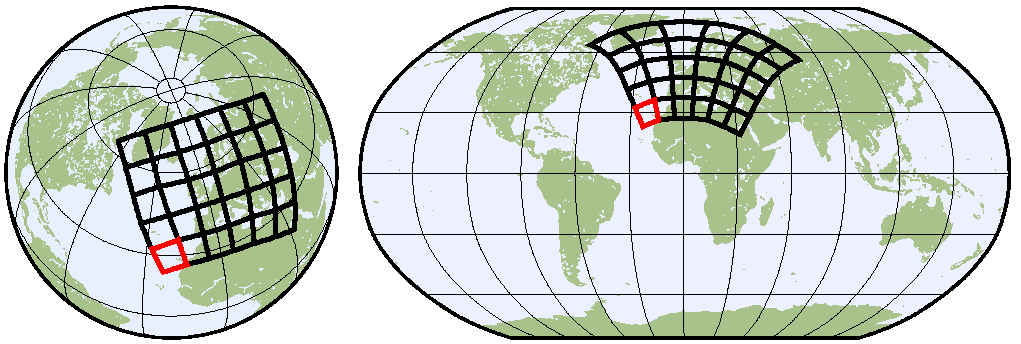
\includegraphics{grids/curv.pdf}}}
}{
{\scalebox{0.99}{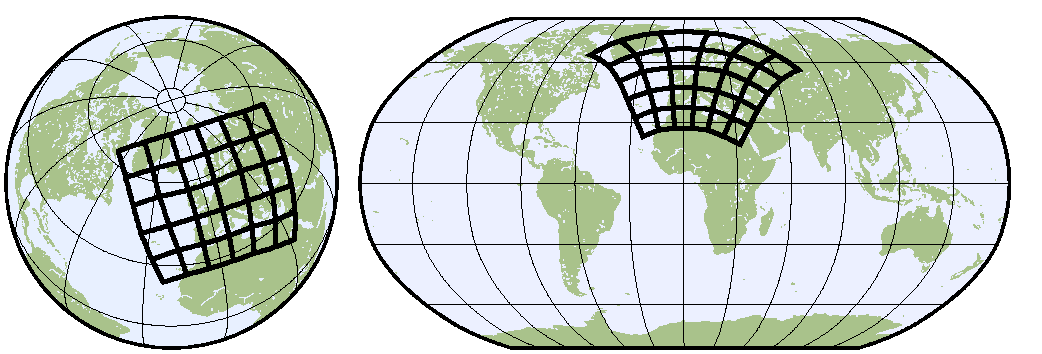
\includegraphics{grids/curv}}}
}
\caption[curvgrid]{Orthographic and Robinson projection of the
  curvilinear grid,  the first grid cell is colored red}
\end{figure}

\newpage
\section{Example description for an unstructured grid}
Here is an example of the {\CDO} description for an unstructured grid.
xvals/yvals describes the position of 30 independent hexagonal grid cells.
The first 6 values of xbounds/ybounds are the corners of the first
grid cell. The first grid cell is colored red.
\begin{lstlisting}[frame=single, backgroundcolor=\color{pyellow}, basicstyle=\footnotesize]
gridtype  = unstructured
gridsize  = 30
nvertex   = 6
xvals     =  |-36|   36    0  -18   18  108   72   54   90  180  144  126  162 -108 -144 
            -162 -126  -72  -90  -54    0   72   36  144  108 -144  180  -72 -108  -36 
xbounds   =  |339    0    0  288  288  309|        21   51   72   72    0    0
               0   16   21    0  339  344       340    0   -0  344  324  324
              20   36   36   16    0    0        93  123  144  144   72   72
              72   88   93   72   51   56        52   72   72   56   36   36
              92  108  108   88   72   72       165  195  216  216  144  144
             144  160  165  144  123  128       124  144  144  128  108  108
             164  180  180  160  144  144       237  267  288  288  216  216
             216  232  237  216  195  200       196  216  216  200  180  180
             236  252  252  232  216  216       288  304  309  288  267  272
             268  288  288  272  252  252       308  324  324  304  288  288
             345  324  324   36   36   15        36   36  108  108   87   57
              20   15   36   57   52   36       108  108  180  180  159  129
              92   87  108  129  124  108       180  180  252  252  231  201
             164  159  180  201  196  180       252  252  324  324  303  273
             236  231  252  273  268  252       308  303  324  345  340  324
yvals     =   |58|   58   32    0    0   58   32    0    0   58   32    0    0   58   32 
               0    0   32    0    0  -58  -58  -32  -58  -32  -58  -32  -58  -32  -32 
ybounds   =   |41   53   71   71   53   41|        41   41   53   71   71   53
              11   19   41   53   41   19       -19   -7   11   19    7  -11
             -19  -11    7   19   11   -7        41   41   53   71   71   53
              11   19   41   53   41   19       -19   -7   11   19    7  -11
             -19  -11    7   19   11   -7        41   41   53   71   71   53
              11   19   41   53   41   19       -19   -7   11   19    7  -11
             -19  -11    7   19   11   -7        41   41   53   71   71   53
              11   19   41   53   41   19       -19   -7   11   19    7  -11
             -19  -11    7   19   11   -7        11   19   41   53   41   19
             -19   -7   11   19    7  -11       -19  -11    7   19   11   -7
             -41  -53  -71  -71  -53  -41       -53  -71  -71  -53  -41  -41
             -19  -41  -53  -41  -19  -11       -53  -71  -71  -53  -41  -41
             -19  -41  -53  -41  -19  -11       -53  -71  -71  -53  -41  -41
             -19  -41  -53  -41  -19  -11       -53  -71  -71  -53  -41  -41
             -19  -41  -53  -41  -19  -11       -19  -41  -53  -41  -19  -11
\end{lstlisting}

\begin{figure}[b]

\ifpdfoutput{
{\scalebox{1}{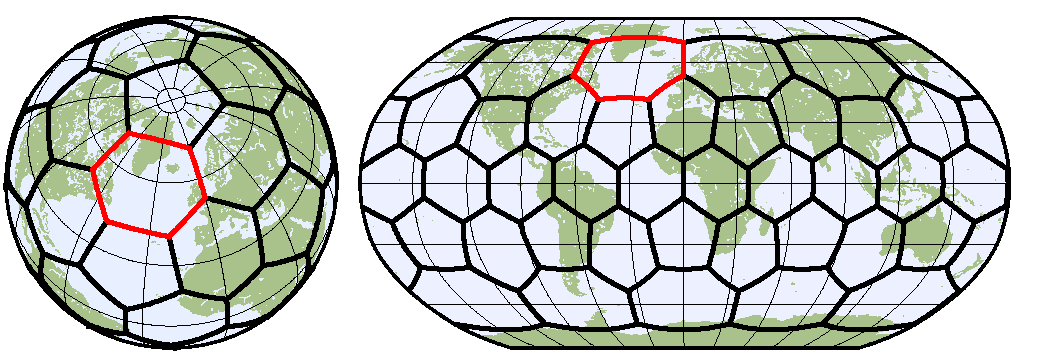
\includegraphics{grids/cell.pdf}}}
}{
{\scalebox{1}{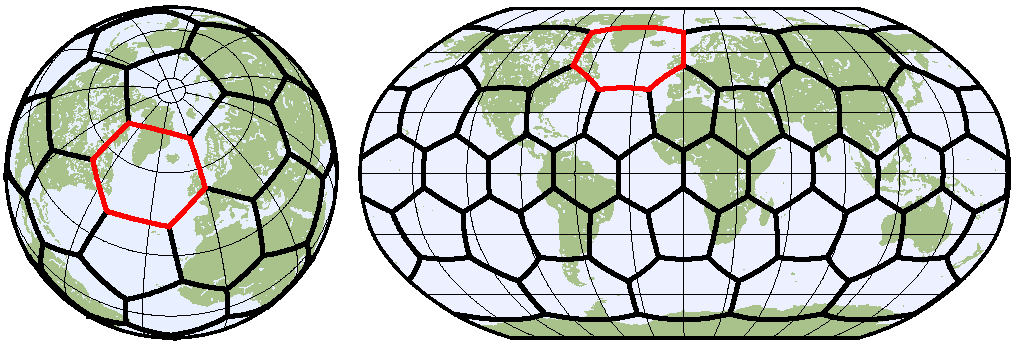
\includegraphics{grids/cell}}}
}
\caption[cellgrid]{Orthographic and Robinson projection of the unstructured grid}
\end{figure}

%%% Local Variables: 
%%% mode: latex
%%% TeX-master: "grid"
%%% End: 


\clearpage
\ifpdfx
\phantomsection
\addcontentsline{toc}{chapter}{\indexname}
\printindex
\else
\input{catalog}
\input{alphabetic_list}
\fi
\end{document}
